% Generated by benchmark.py
% Requires booktabs, graphicx, float in your preamble.

\begin{table}[H]
  \centering\small
  \setlength{\tabcolsep}{6pt}
  \caption{Models tested: model name, node count (before distribution), and preview.}
  \label{tab:rt-scene-overview}
  \begin{tabular}{@{}lrl@{}}
    \toprule
    \textbf{Model} & \textbf{Nodes} & \textbf{Preview} \\
    \midrule
    \texttt{artemis} & 29 & 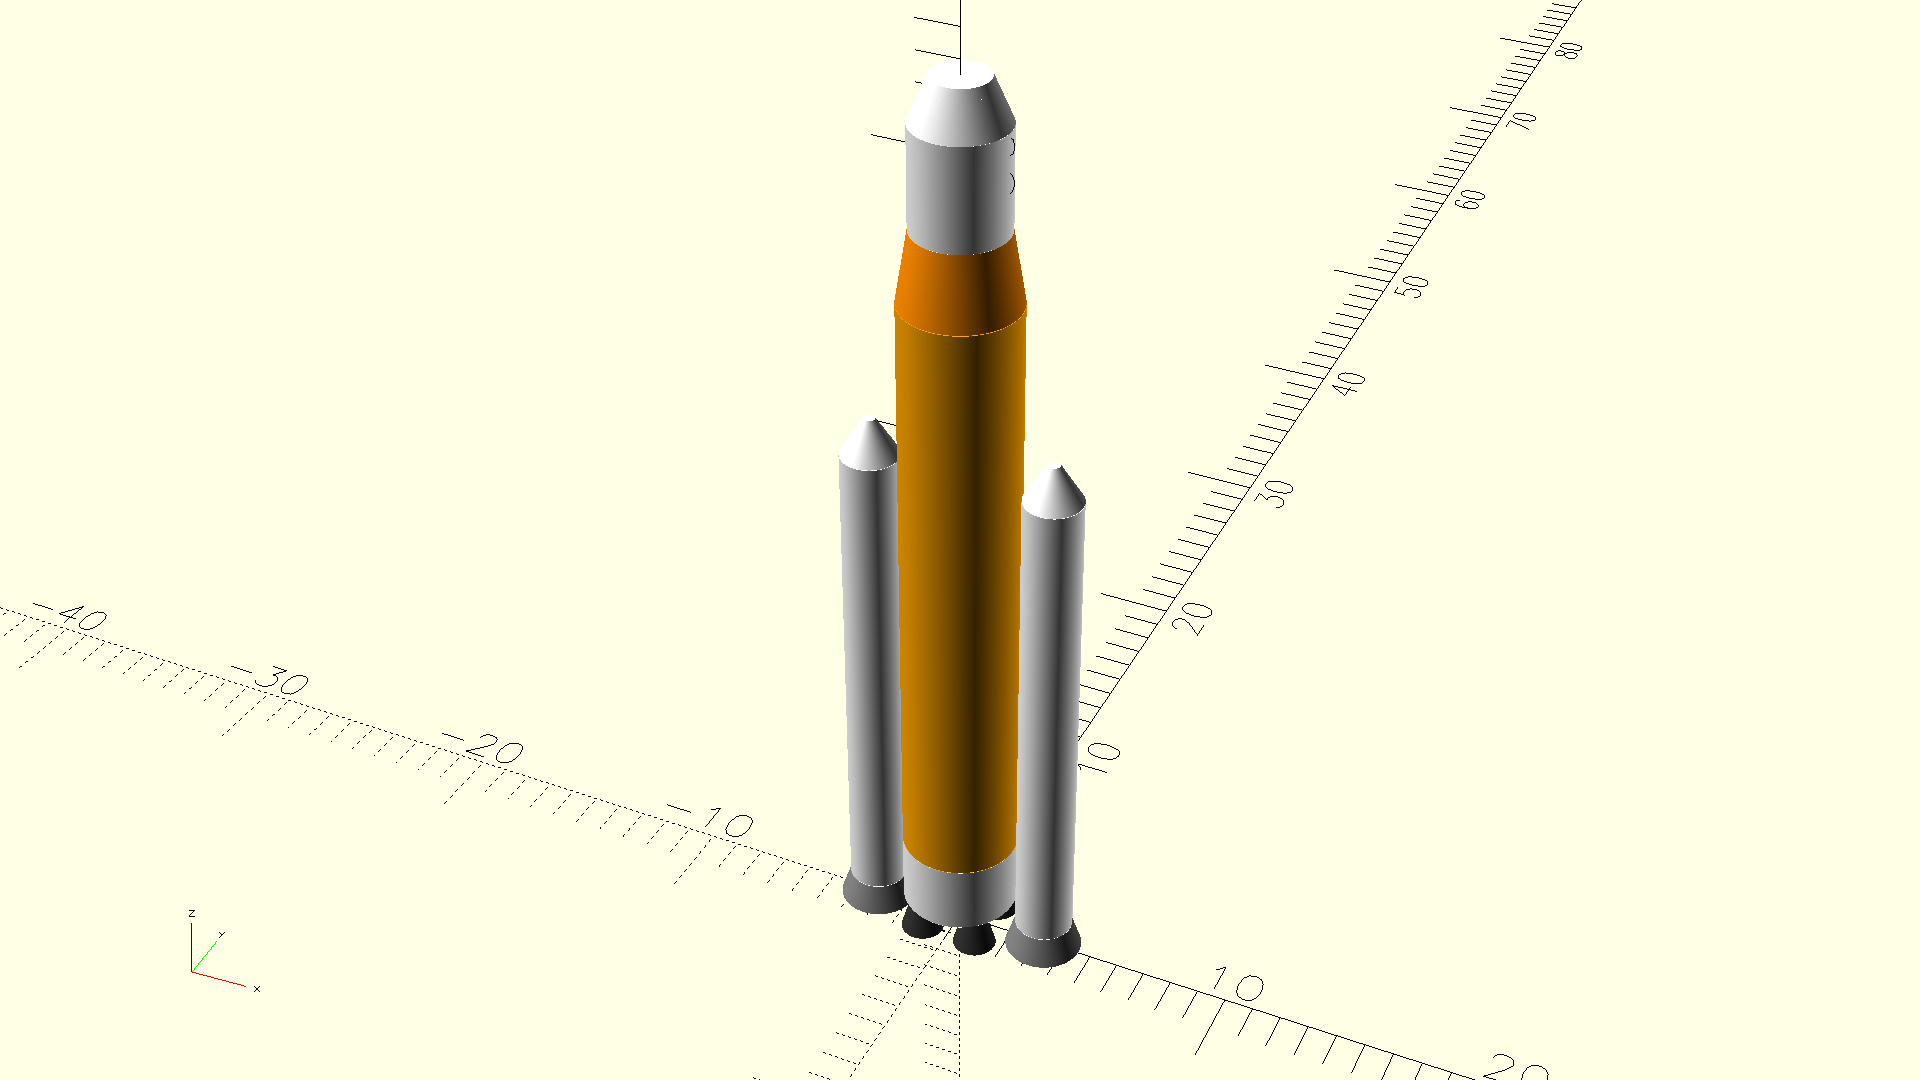
\includegraphics[height=2.8cm]{bench_20260428_204450/artemis/frame.png} \\
    \texttt{distribution\_stress} & 39999 & 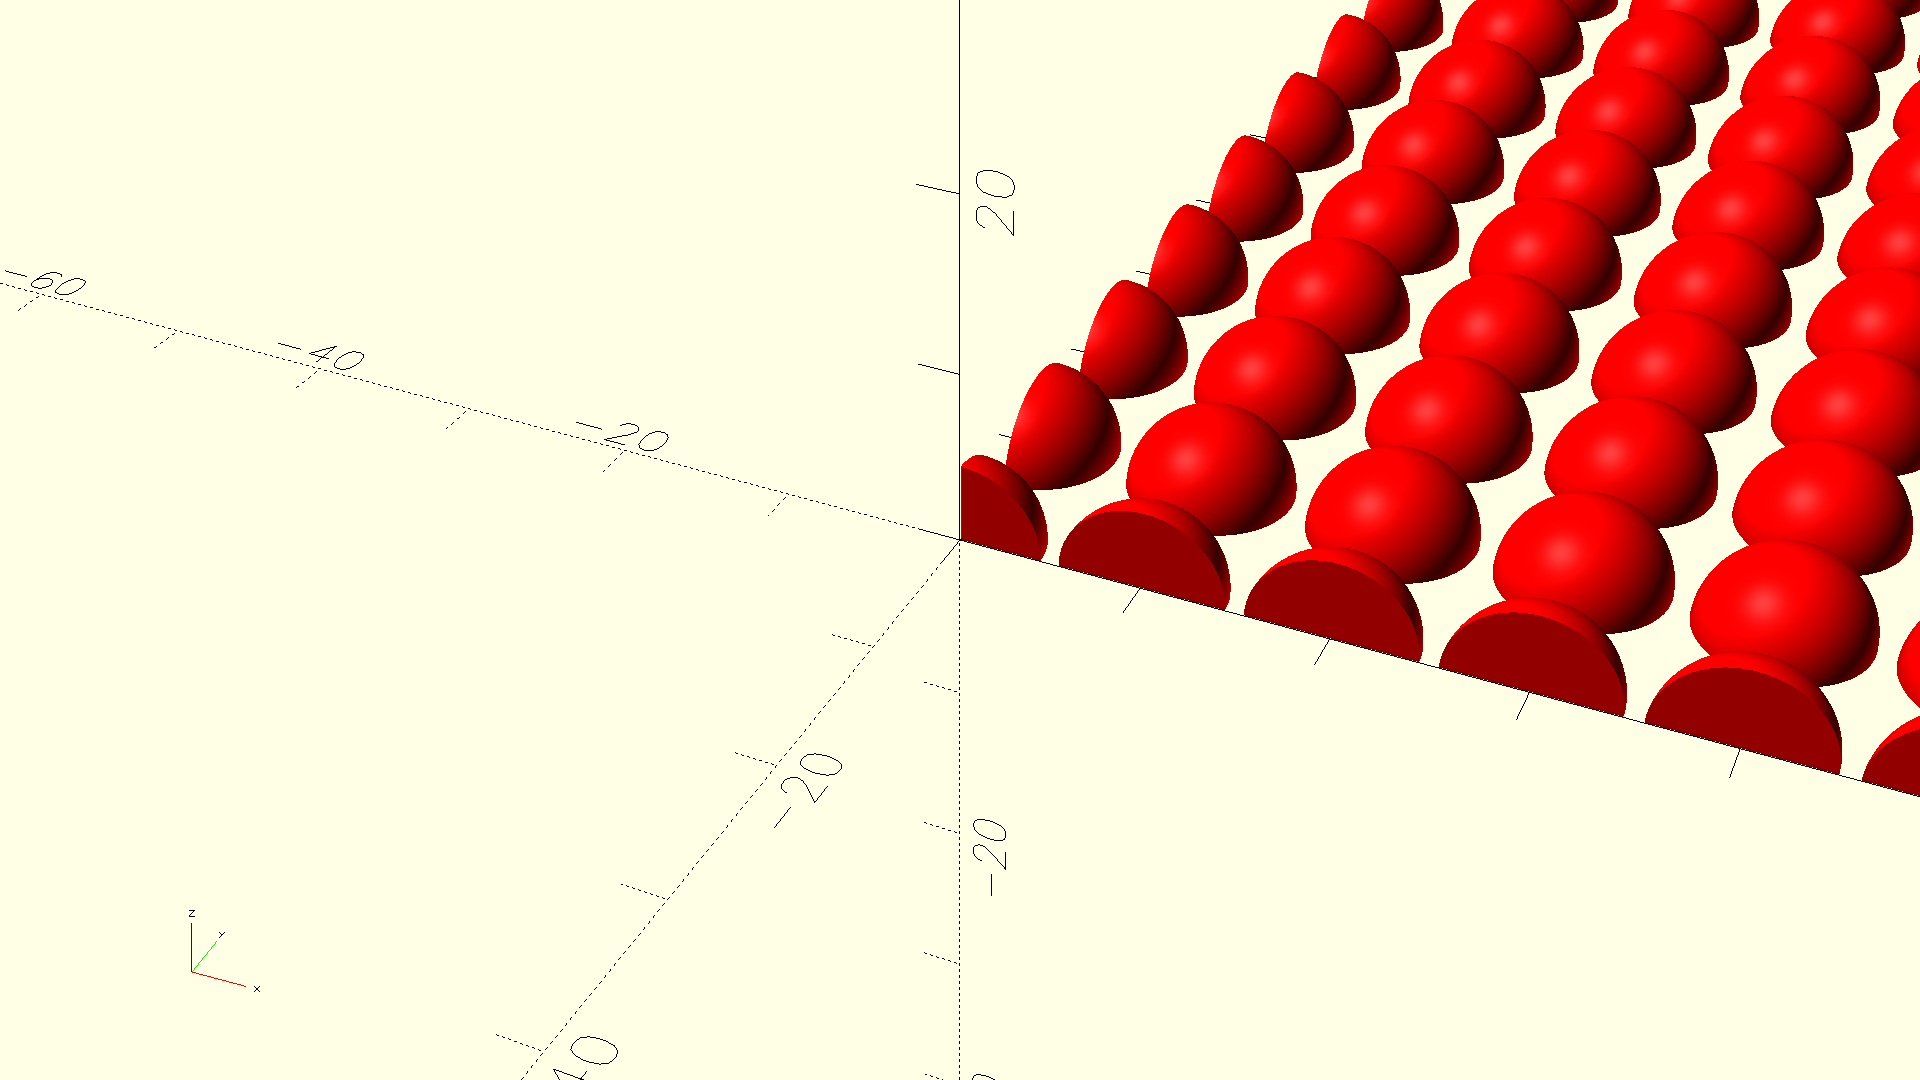
\includegraphics[height=2.8cm]{bench_20260428_204450/distribution_stress/frame.png} \\
    \texttt{mechanical\_piece} & 675 & 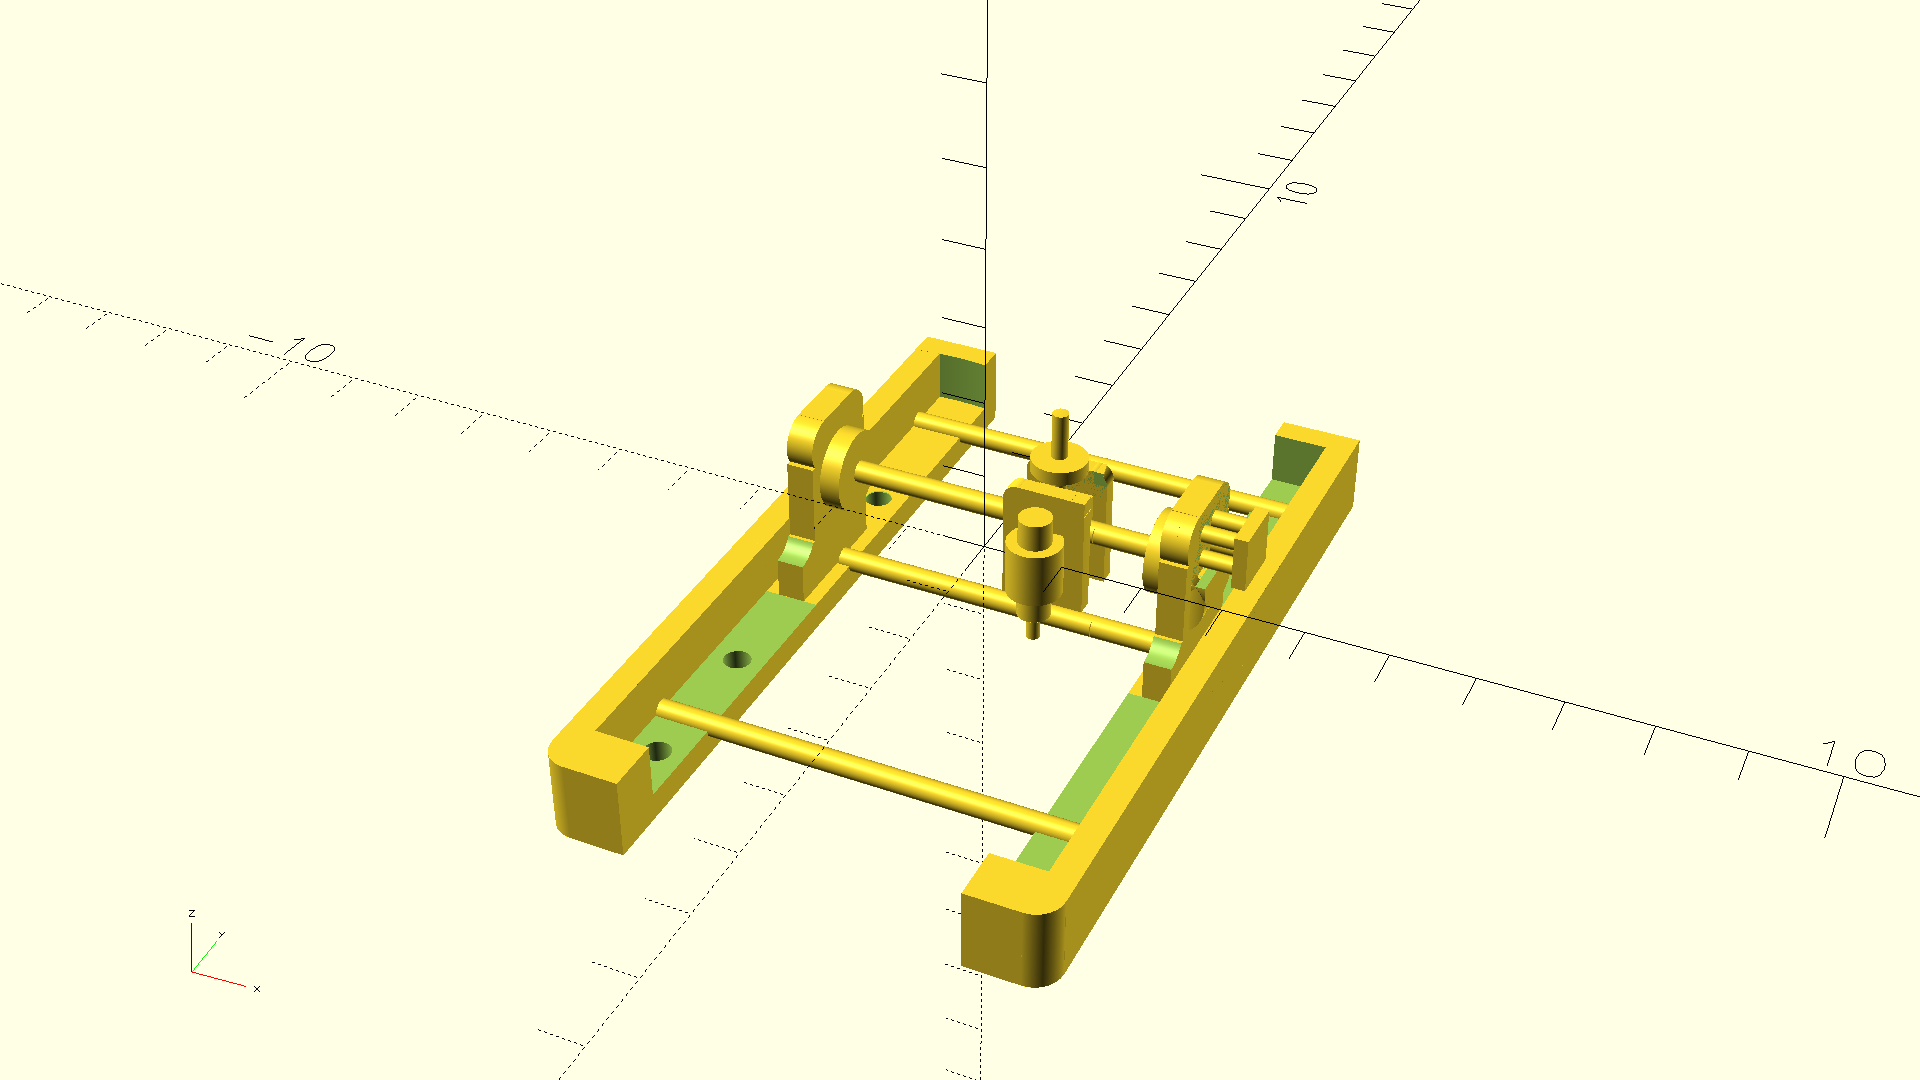
\includegraphics[height=2.8cm]{bench_20260428_204450/mechanical_piece/frame.png} \\
    \texttt{menger\_sponge} & 15999 & 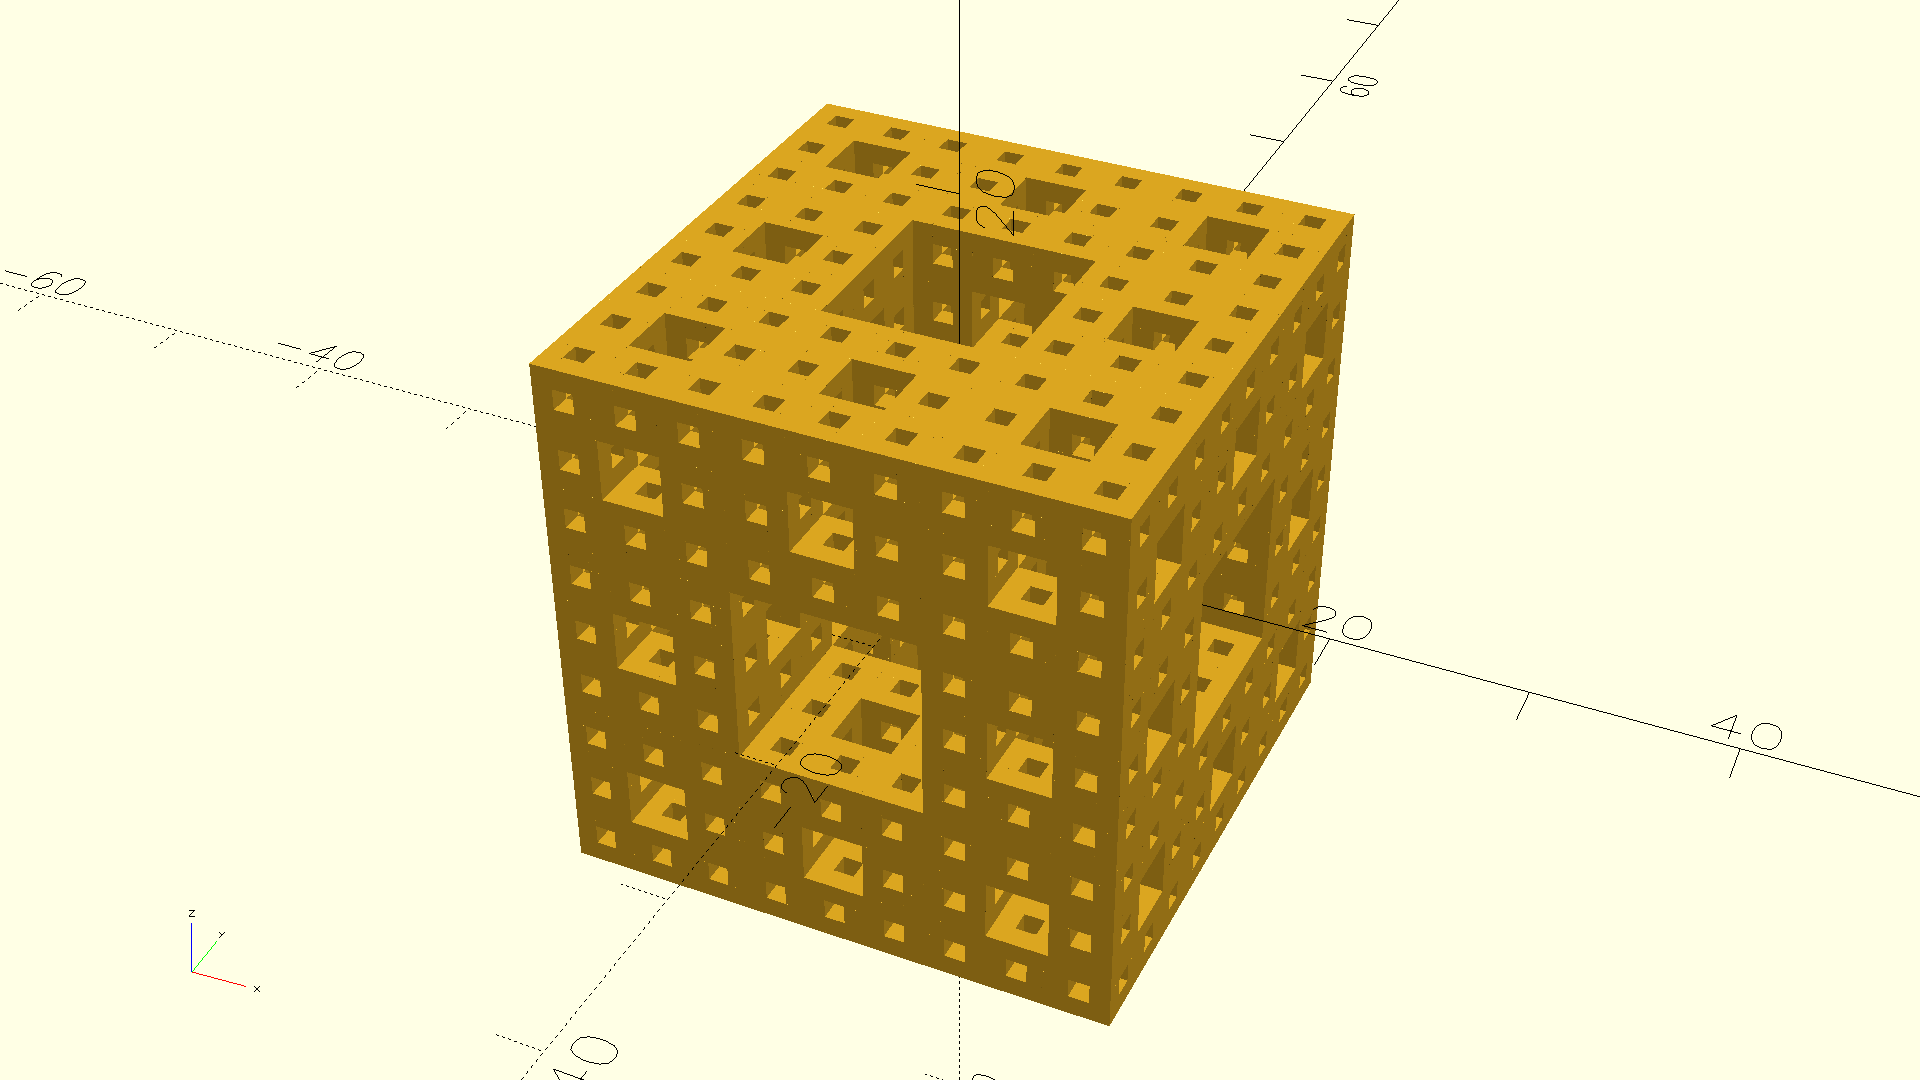
\includegraphics[height=2.8cm]{bench_20260428_204450/menger_sponge/frame.png} \\
    \texttt{shuffled\_spheres} & 1349 & 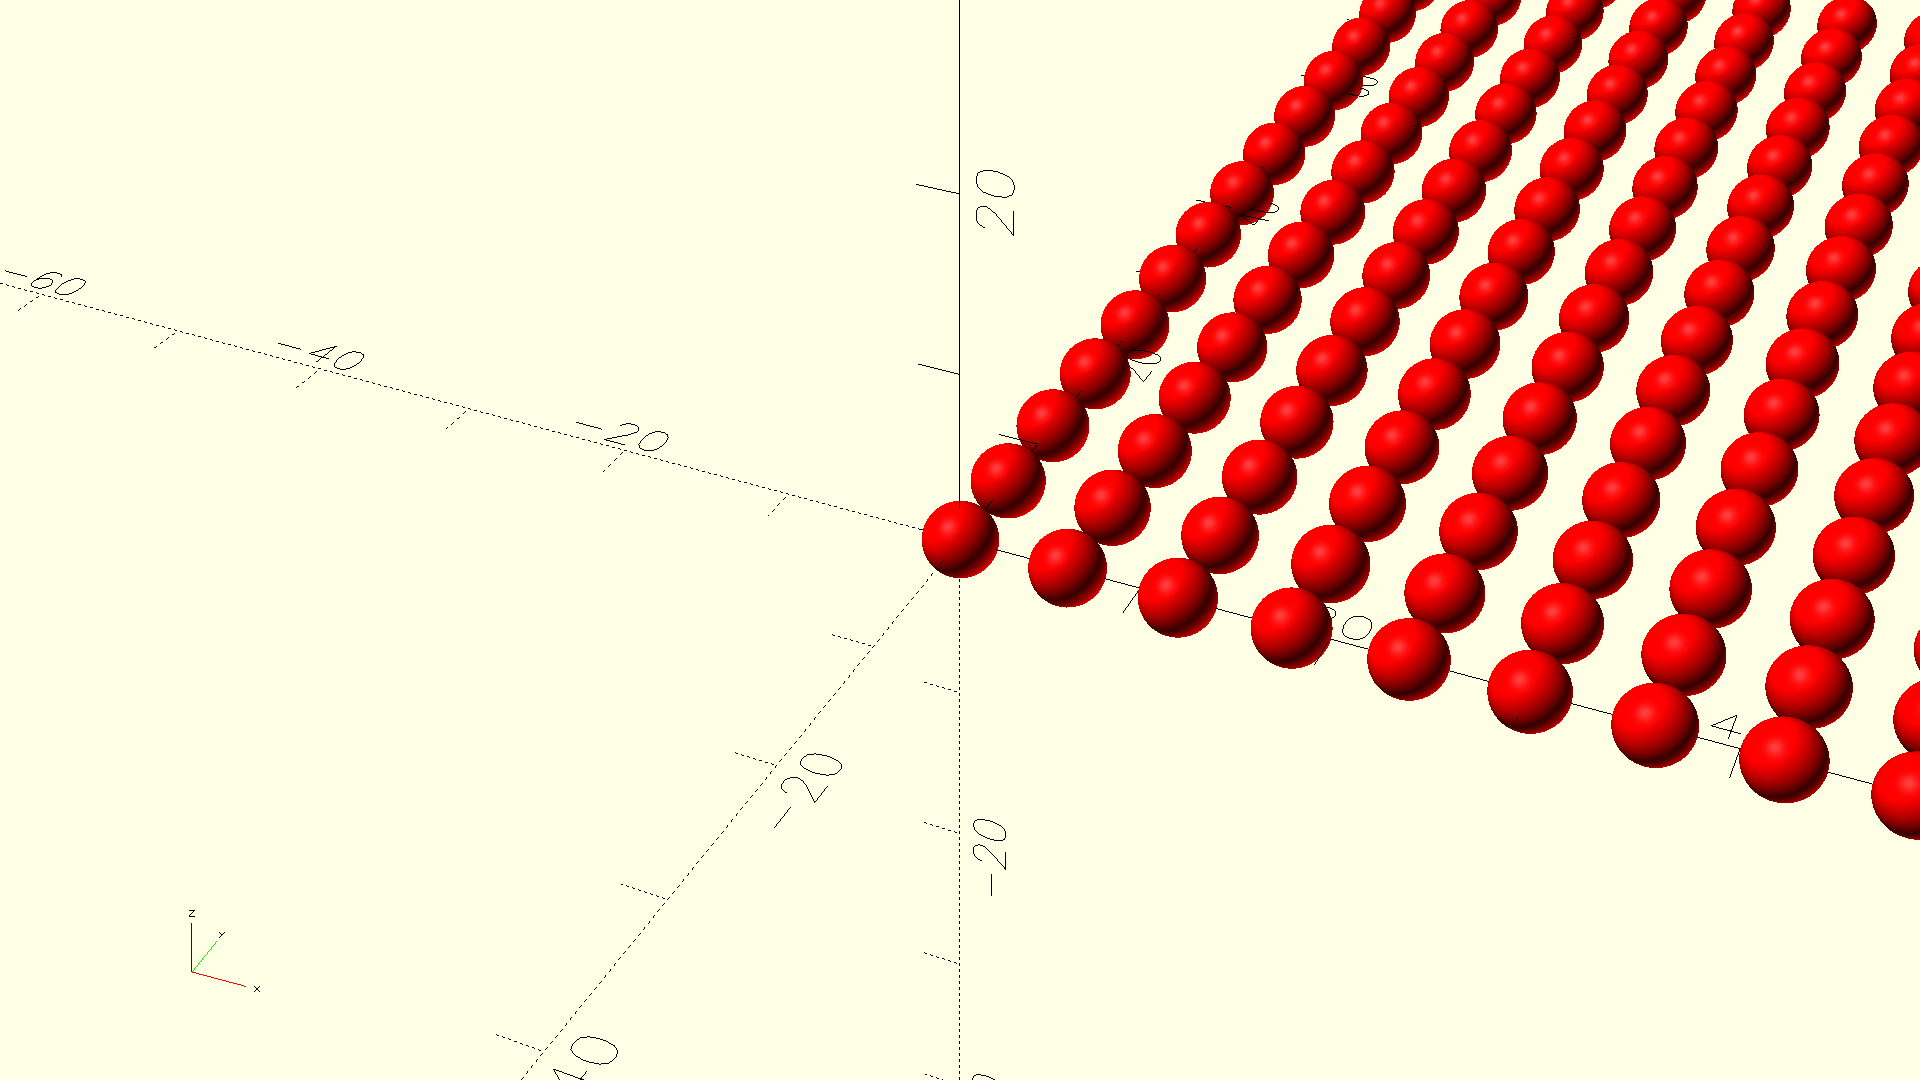
\includegraphics[height=2.8cm]{bench_20260428_204450/shuffled_spheres/frame.png} \\
    \texttt{sierpinski} & 8191 & 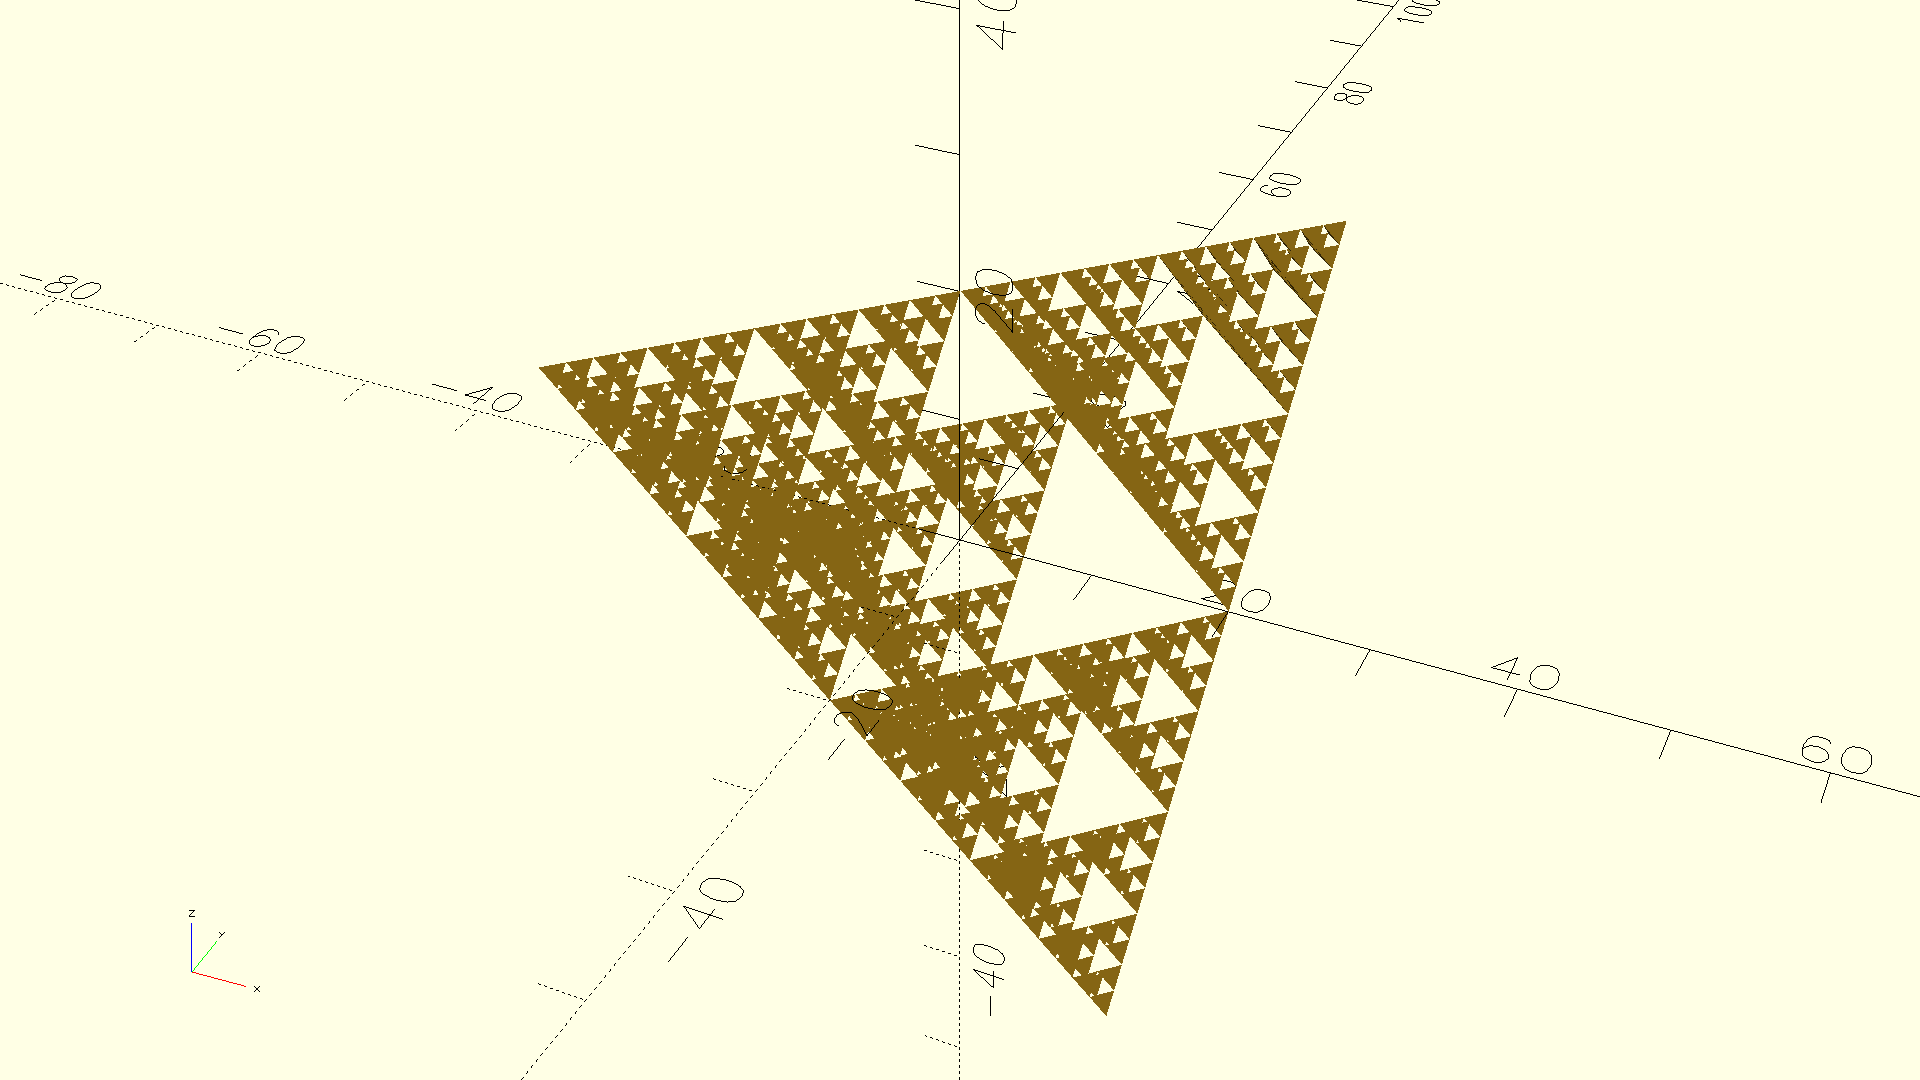
\includegraphics[height=2.8cm]{bench_20260428_204450/sierpinski/frame.png} \\
    \texttt{sphere\_stress} & 15999 & 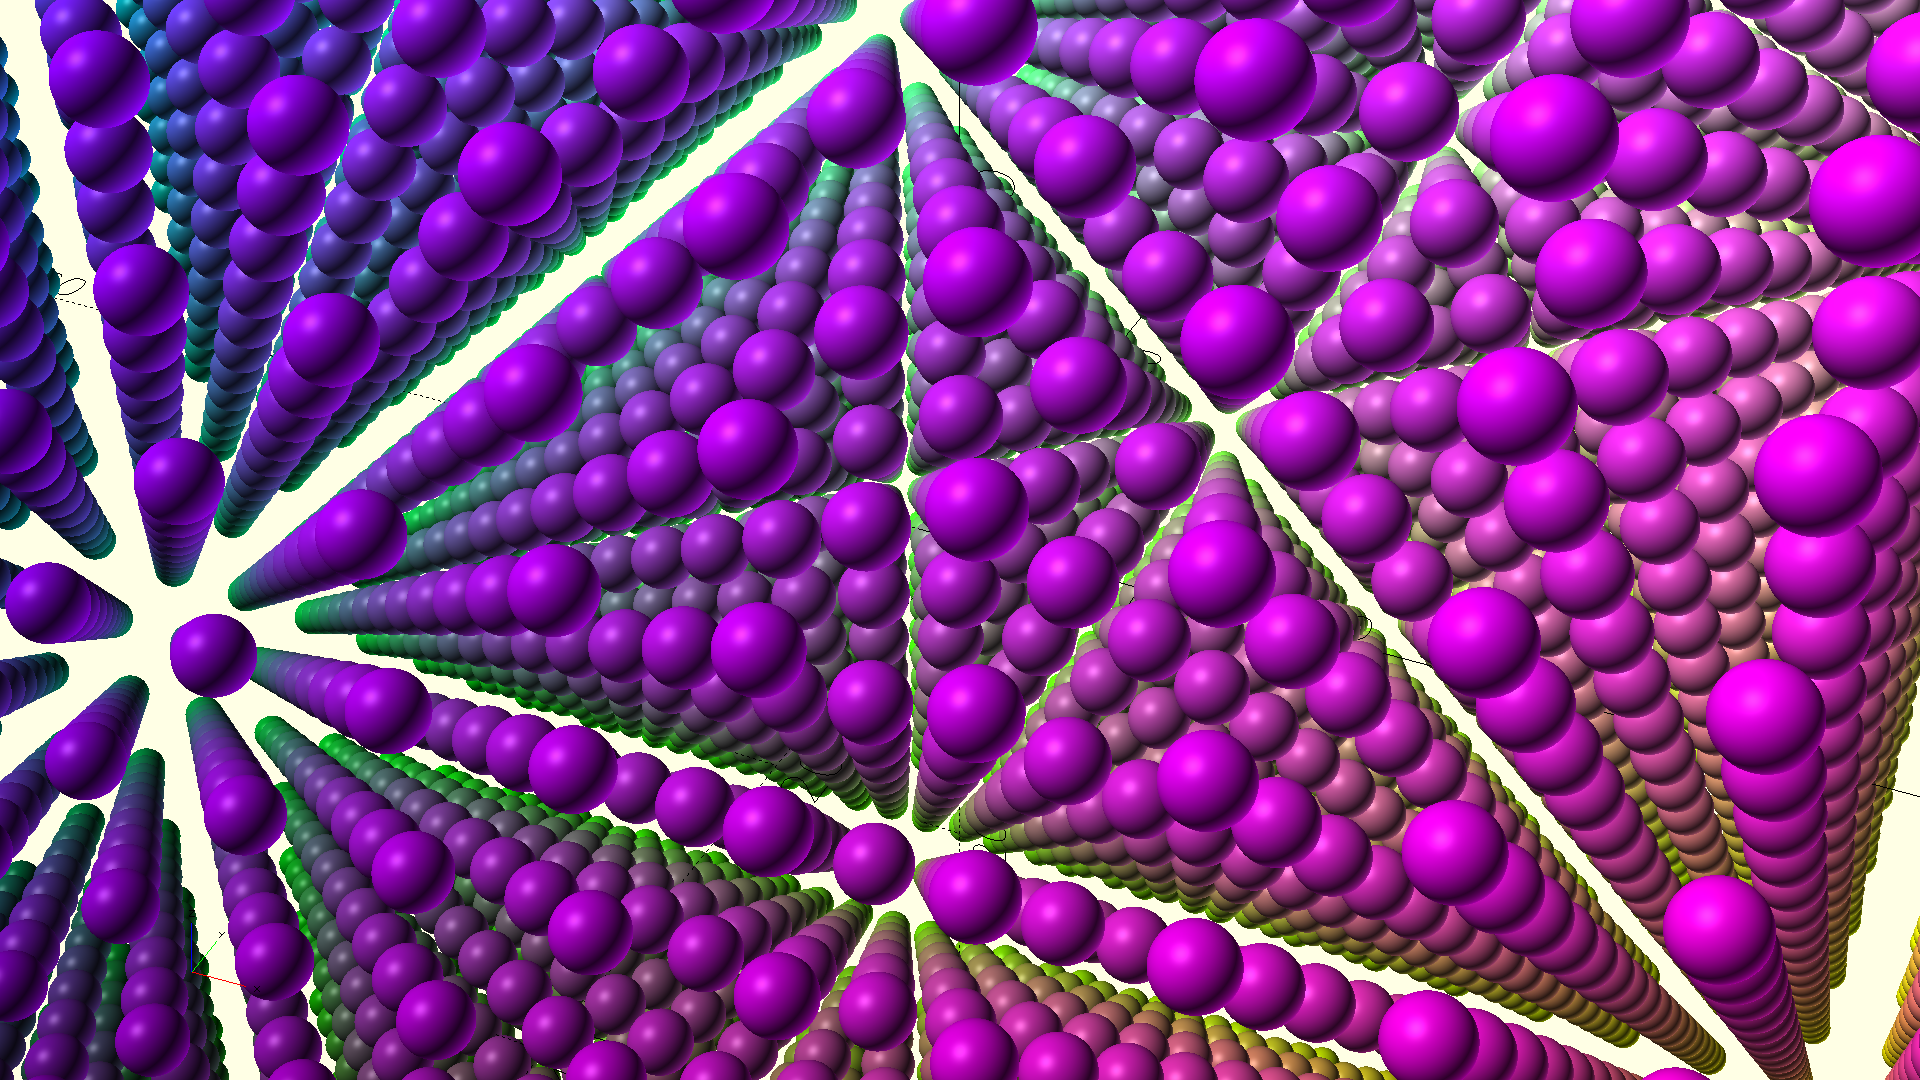
\includegraphics[height=2.8cm]{bench_20260428_204450/sphere_stress/frame.png} \\
    \bottomrule
  \end{tabular}
\end{table}
